\documentclass[12pt,a4paper,oneside,ngerman]{article}
\usepackage[utf8]{inputenc}
\usepackage{color}
\usepackage{tikz}
\usepackage{amsmath}
\usepackage{amssymb}
\usepackage{calc}
\usepackage{mathtools}
\usepackage{float}
\usepackage{struktex}
\usepackage{ulem}
\usepackage{pdfpages}
\usepackage{listings}

\title{EZS}
\author{Simon Krücken}

\newcommand\tab[1][1cm]{\hspace*{#1}}

\begin{document}
    
\begin{titlepage}
%    \maketitle
\end{titlepage}
\tableofcontents


\section[Standard Fragen]{Standard Frage}

1. Wo mit Beschäftigt sich IT-Sicherheit(Definition)?\\
IT-Sicherheit beschäftigt sich mit der Vorbeugung, dem Erkennen und der Reaktion auf Ereignisse, die die Integrität der Daten, die Nutzbarkeit der Systeme und die (digitale) Privatsphäre gefährden.\\

2. Vor welchen drei Gefährdungen müssen Rechner- und Netzwehrkomponenten geschützt werden?\\
\begin{itemize}
	\item Spionage
	\item Sabotage
	\item Missbrauch
\end{itemize}

3. Nennen Sie die in der Vorlesung genannten drei Schutzziele für Rechner- und Netzkomponenten.\\
\begin{itemize}
	\item Vertraulichkeit
	\item Integrität
	\item Verfügbarkeit
\end{itemize}

\section{Eigener Verschlüsslungs Algo.}
12 Stellige Passwörter werden nach dem Muster abuvcdwxefyz gebildet.
Wobei uvwxyz der Passwort Kern \*\&asz6K\* ist. und \*ab\* die ersten beiden Buchstaben der url entsprechen.
\*cd\* den dritten und vierten Buchstaben welche um ROT+1 verschoben sind. Und schlussendlich \*ef\* die letzten beiden Buchstaben welche
um ROT-1 verschoben sind. URLs Kürzer als 6 zeichen werden einfach wiederholt.\\

www.heise.de =$>$ heiseh\\
abuvcdwxefyz\\
he\&ajtszdg6K\\

\section{Dateirechte}
Dateirechte so setzten das sie Superuser Rechte hat auch wenn sie nicht als Superuser gestartet wurde.
\begin{lstlisting}
	sudo chown root:root get_pic
\end{lstlisting}

Datei /usr/local/bin/backup nur für Besitzer $>$local$<$ lesbar, schreibbar und ausführbar machen. Die Gruppe $>$its$<$ soll die Datei nur ausführen dürfen.
\begin{lstlisting}
	chown local /usr/local/bin/backup
	chgrp its /usr/local/backup
	chmod 710 /usr/local/bin/backup
\end{lstlisting}


\section{Anhang}

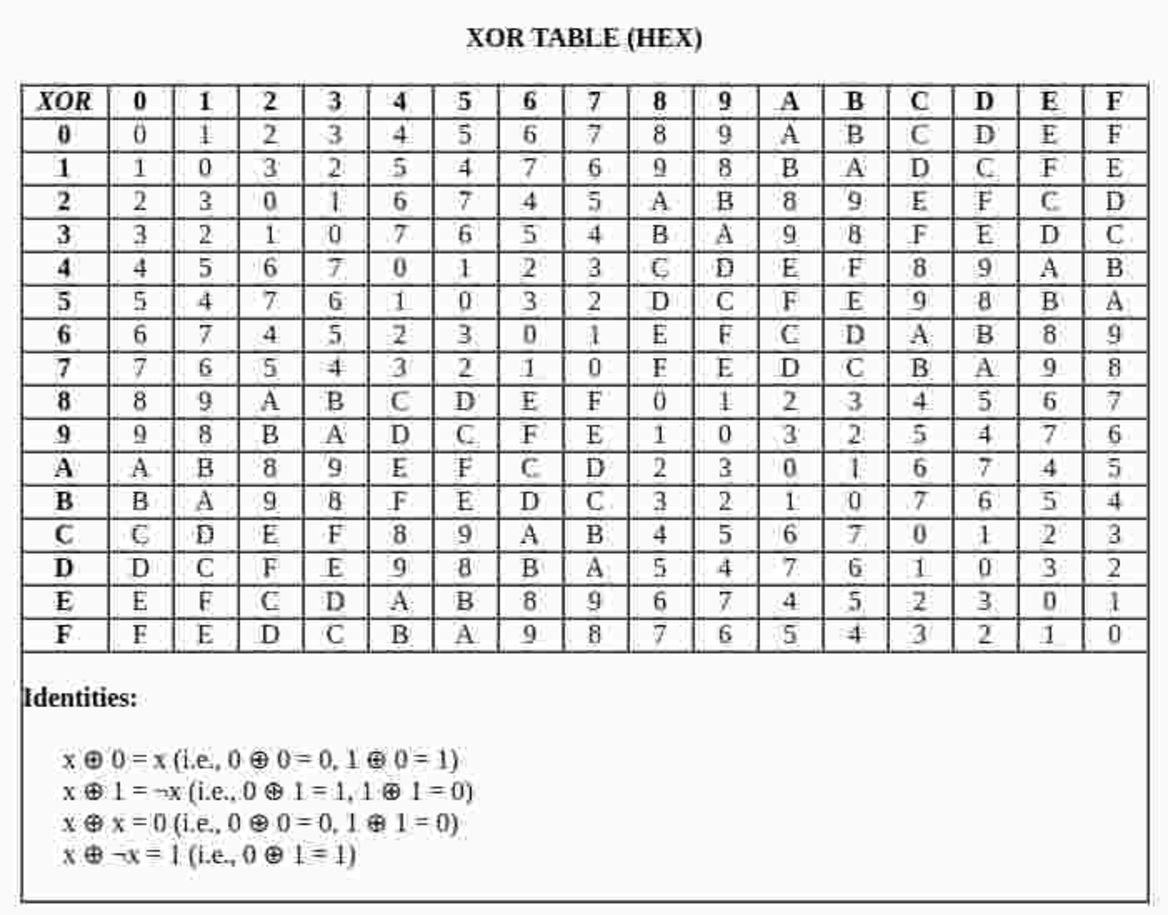
\includepdf[scale=0.8]{xor_tabelle.pdf}

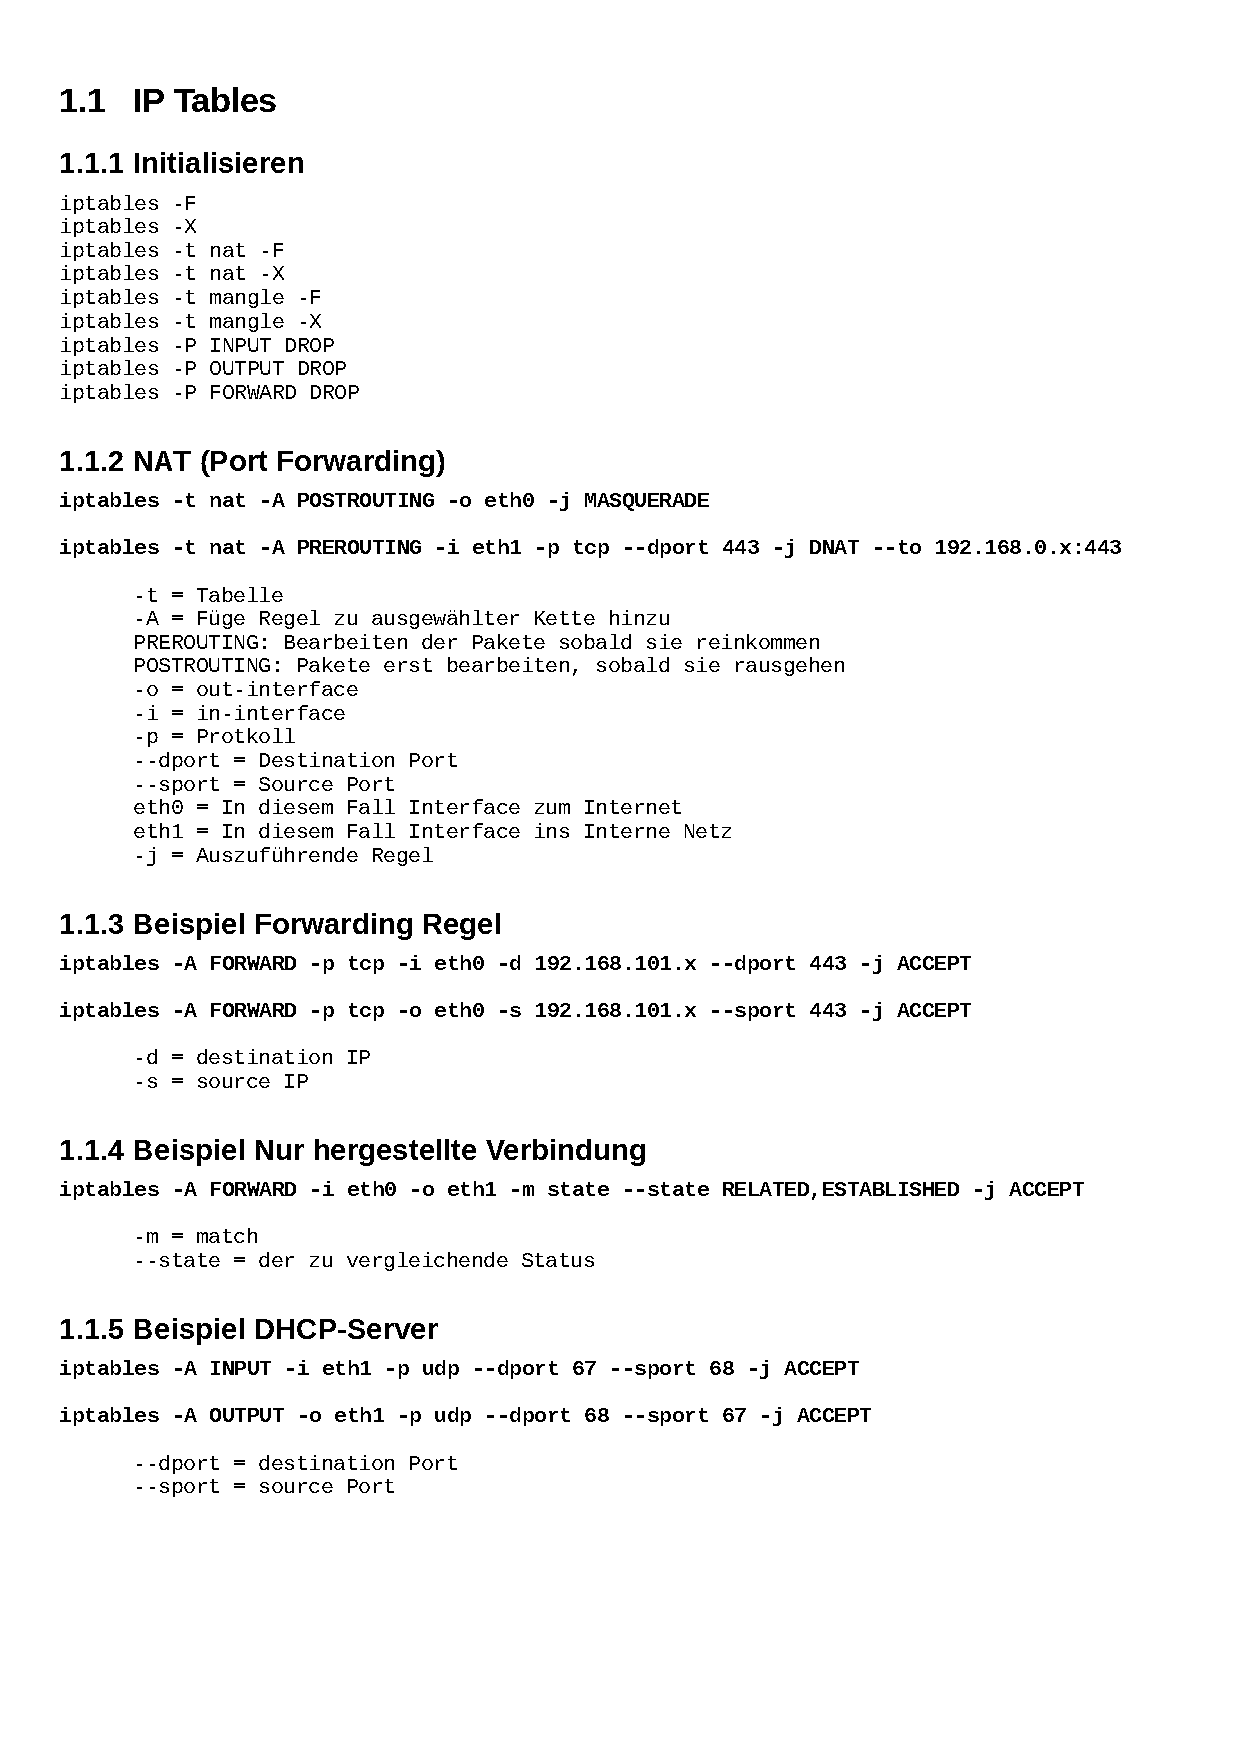
\includepdf[pages={1,2}]{hilfsblatt_eck.pdf}

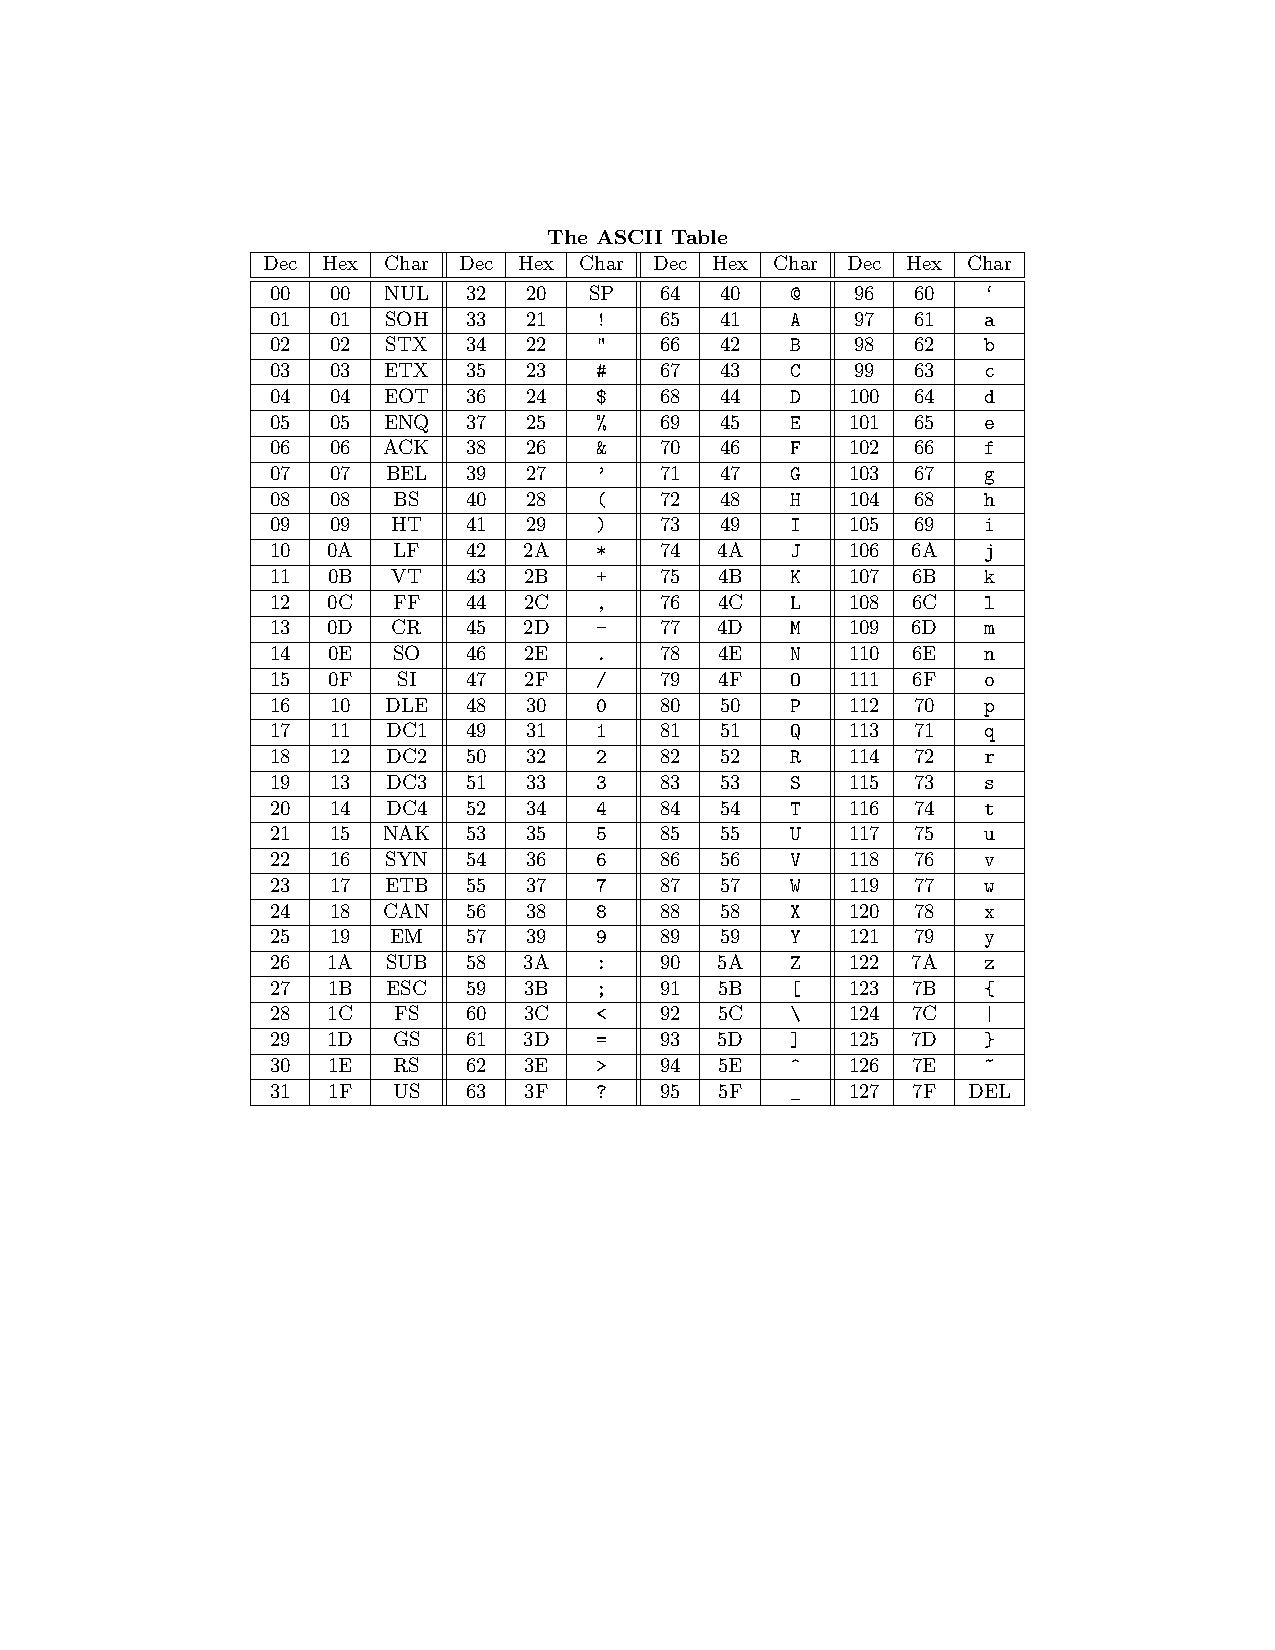
\includepdf[scale=1.2]{ascii_tabelle.pdf}

\end{document}